\documentclass[10pt,a4paper]{article}
\usepackage[margin=2.2cm]{geometry}
\usepackage{fontspec}
\usepackage{kotex}
\setmainfont{Apple SD Gothic Neo}
\setsansfont{Apple SD Gothic Neo}
\usepackage{amsmath,amssymb}
\usepackage{graphicx}
\usepackage{booktabs}
\usepackage{caption}
\usepackage[dvipsnames]{xcolor}
\usepackage[colorlinks=true,linkcolor=MidnightBlue,citecolor=MidnightBlue,
            urlcolor=MidnightBlue]{hyperref}
\usepackage{titlesec}
\titleformat{\section}{\large\bfseries}{\thesection}{0.6em}{}
\titleformat{\subsection}{\normalsize\bfseries}{\thesubsection}{0.5em}{}
\captionsetup{font=small,labelfont=bf}
\setlength{\parskip}{0.35em}
\setlength{\parindent}{0pt}

% 주장 상자 — 모든 주장은 반증 조건을 함께 적는다
\usepackage{mdframed}
\newmdenv[linewidth=0.4pt,linecolor=gray!60,backgroundcolor=gray!5,
          innertopmargin=6pt,innerbottommargin=6pt,skipabove=8pt,skipbelow=8pt]{claimbox}
\newcommand{\claim}[2]{\begin{claimbox}\textbf{주장.} #1\par\smallskip
  \textcolor{gray!70}{\textbf{반증 조건.} #2}\end{claimbox}}

\title{\bfseries 위약을 통과해도 새 정보가 아닐 수 있다\\[2pt]
\large 판정의 세 번째 관문}
\author{월드모델 실험실 · 노트 650--651}
\date{2026-08-05}
\begin{document}\maketitle

\section{한 줄}

새 축이 **위약**을 이겼다. 그런데 새 정보가 아니었다 --- 판에 **이미 있던 축의
사본**이었다. 위약은 그 축의 값을 섞은 것이라, *다른 축이 같은 것을 이미
갖고 있는지*는 원리적으로 못 본다.

\section{어쩌다 알게 됐나}

노트 649 가 규칙을 하나 냈다. 범도메인 상태 축이 서려면 같은 날짜라도
\textbf{대상마다 값이 달라야} 한다 --- 상태는 시간이 아니라 (시간 $\times$ 대상)
으로 들어와야 한다. 전국 이동량 축이 수준 $\cdot$ 차분 $\cdot$ 추세제거 세
변형에서 모두 실패했고($-0.0211$ $\cdot$ $-0.0177$ $\cdot$ $-0.0092$, 전부 0/12),
실패 무늬가 \emph{축 내용과 무관했기} 때문이다.

노트 650 이 그 규칙으로 축을 지었다. \verb|crowd_share| --- 이 작품 직전 90일에
같은 갈래로 나온 작품의 몫. 수집 비용이 0 이고 가중 덮음 0.629, 실제 부착
13,635 행이다. 판정은 이랬다.

\begin{center}\small
\begin{tabular}{lrr}\toprule
팔 & 판 차 & 양수 \\ \midrule
혼잡도 & $-0.0007$ & 4/12 \\
위약(갈래만 섞음) & $-0.0028$ & 0/12 \\ \midrule
\textbf{신호 몫} & $\mathbf{+0.0021}$ & \\ \bottomrule
\end{tabular}\end{center}

\claim{위약보다 나으므로 축이 정보를 나른다.}{다른 축이 같은 정보를 이미
갖고 있으면 이 부등호는 성립하면서도 새 정보는 0 이다.}

부등호가 뒤집힌 것은 이 판에서 처음이었다. 날씨 축은 위약($-0.0344$)이
진짜($-0.0283$)보다 \emph{나빴고}, 그것이 ``신호가 아니라 차원 비용'' 판정의
근거였다(노트 640). 그래서 노트 650 을 ``상태 축이 처음으로 위약을 이겼다''
로 적었다.

\section{창을 바꿔 보니 아무것도 안 바뀌었다}

신호가 왜 문턱의 절반뿐인지 가르려고 창 길이를 바꿨다. 혼잡도가 실재하면
30일 창과 365일 창은 다른 것을 재야 한다. \textbf{선택은 학습 행에서만} 하고
유보는 안 봤다(노트 568).

\begin{center}\small
\begin{tabular}{lrrrrrr}\toprule
창(일) & 30 & 60 & 90 & 120 & 180 & 365 \\ \midrule
$|\rho|$ 축 vs 라벨 & .1243 & .1247 & .1279 & .1286 & .1294 & .1334 \\ \bottomrule
\end{tabular}\end{center}

최대/최소 $=$ \textbf{1.07} 이다. 창을 12배 늘려도 움직이지 않는다.

\section{그런데 잡음도 아니었다}

사전 등록에 ``창에 둔감하면 잡음''이라고 적었는데 \textbf{그 이분법이 좁았다}.
$|\rho| = 0.13$ 은 잡음이라기엔 크다. 창에 불변이라는 것은 축이 \emph{최근
혼잡}이 아니라 \textbf{느리게 변하는 무언가}를 잰다는 뜻이다. 직접 확인했다.

\begin{center}\small
\begin{tabular}{lrrrrr}\toprule
& 게임 & 만화 & 모바일 & 세계애니 & 애니 \\ \midrule
창 30 $\leftrightarrow$ 365 자기상관 & $+.877$ & $+.873$ & $+.886$ & $+.884$ & $+.907$ \\
기존 \verb|gen| 축과 $|\rho|$ & $.819$ & $.512$ & $.804$ & $.417$ & $.665$ \\ \bottomrule
\end{tabular}\end{center}

12배 다른 두 창이 서로 $+0.88$ 이고, 그 축이 이미 판에 있는 \verb|gen| 축과
$0.42\sim0.82$ 다. 이 축은 ``이 시기가 붐볐나''가 아니라 \textbf{``이 작품이 어느
갈래인가''}를 다르게 적은 것이었다. 갈래 점유율은 시간에 따라 거의 안 변하므로
창이 애초에 무의미했다.

\section{세 관측이 한꺼번에 설명된다}

\begin{itemize}
\item 라벨과 $|\rho|=0.13$ 인 이유 --- 인기 갈래가 잘 팔린다.
\item 창에 불변인 이유 --- 갈래 점유율이 안정적이다.
\item 판 이득이 $+0.0021$ 뿐인 이유 --- \verb|gen| 이 \textbf{이미 그것을 나른다}.
\end{itemize}

노트 650 의 ``위약을 이겼다''는 관측으로는 맞다. 틀린 것은 그 다음 문장
---\,이긴 몫이 \emph{새 정보}라는 것\,---\,이고, 실제로는 \textbf{같은 정보의
다른 인코딩}이었다.

\section{조항}

\claim{판정의 관문은 셋이다 --- ① 배선 ② 위약 ③ \textbf{기존 축과의 상관}.}
{세 관문을 다 통과했는데도 이득이 다른 축의 재인코딩으로 밝혀지면 이 조항이
불완전한 것이다.}

노트 276 이 겹말 가드를 세워 뒀다. 그런데 그것을 \textbf{새 축을 채택할지
고를 때만} 돌리고 \emph{판정을 해석할 때는} 안 썼다. 위약이 못 보는 자리를
겹말 가드가 보는데, 두 가드가 서로 다른 단계에 놓여 있어서 사이가 비어 있었다.

같은 무늬를 이 판이 여러 번 밟았다 --- 노트 548(상한을 기대값으로) $\cdot$
560(전역 표를 단일 이득으로) $\cdot$ 568(유보 기준선을 상한으로) $\cdot$
584(기준선에 준 노력). \textbf{이번 것은 ``대조군을 통과했으니 새롭다''} 이고,
대조군이 무엇을 통제하는지 안 적어서 생겼다.

\section{닫는 갈래와 남은 길}

출시 혼잡도를 \textbf{레코드 안에서} 만드는 길은 여기서 끝난다. 우리 레코드는
시장 전수가 아니라 표본이라 갈래 점유율 이상을 못 뽑는다. 진짜 혼잡도를
재려면 \textbf{시장 전수 출시 목록}이 밖에서 와야 하고, 그것은 수집 문제다.

(시간 $\times$ 대상) 규칙 자체는 아직 산다 --- 다만 이번 시험이 그것을
\emph{확인}한 것이 아니라 \textbf{시험이 안 된 채로 남았다}는 것이 결론이다.
규칙을 지키면서 \emph{기존 축과 겹치지 않는} 축을 아직 못 만들었다.

\begin{figure}[h]\centering
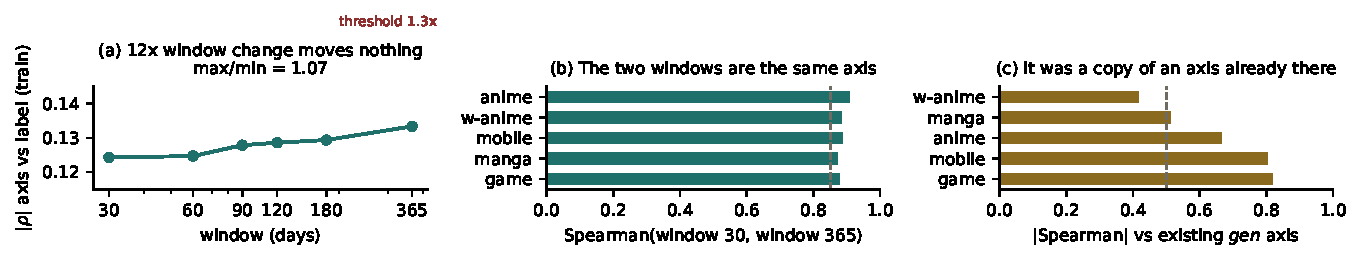
\includegraphics[width=\textwidth]{figs/f1.pdf}
\caption{(a) 창을 12배 늘려도 축$\leftrightarrow$라벨 상관이 안 움직인다
(최대/최소 1.07). (b) 30일 창과 365일 창이 서로 $+0.88$ --- 같은 축이다.
(c) 그리고 이미 판에 있던 \texttt{gen} 축의 사본이었다.}
\end{figure}

\end{document}
